\subsection{Day 3} \label{sec:day3}

The daily meeting took place as planned at 11:00 PST.\footnote{\url{https://confluence.lsstcorp.org/display/DM/OPS+Rehearsal+\%28Day+3\%3A+2020-07-30\%29+Meeting+notes}}

Observations were attempted to repeat images with the previous night's setup.  There was a
disk write timeout from the DAQ.  This was mitigated, the exposure counter was incremented
and a restart allowed the completion of the sequences.  It was noted that this
problem will likely go away once SSDs are installed for the DAQ storage hardware.

Transfers required 2 hours, 50~s for the first image and then downhill from there.
Processing proceeded without incident and all calibrations went to the correct
registry.

Quality analyses show huge differences in darks between nights but this has been
traced to the wrong bias frames (those from 2 weeks prior) being applied.


\begin{figure}
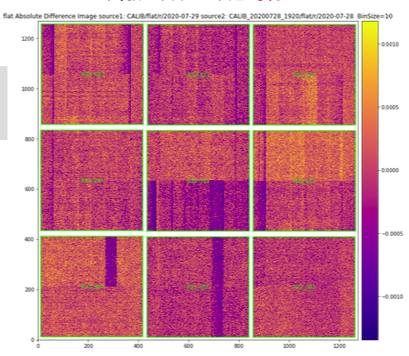
\includegraphics[width=0.45\textwidth]{figures/n3-2bad}
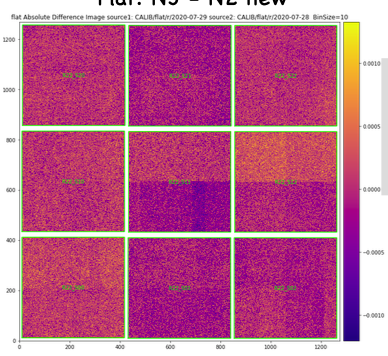
\includegraphics[width=0.43\textwidth]{figures/n3-2}
	\caption{Difference between night two and night three flats with incorrect bias(left),  correct bias subtraction (right).\label{fig:d3}}
\end{figure}


\subsubsection{Discussion}

The rehearsal was deemed finished, except for some follow-on analyses and
the production of this report.  Most discussion revolved around the soonest that
a subsequent rehearsal should be planned (even if it were to repeat this
exercise) and what changes we should plan for.  The current thought is that we
should begin discussing this in September and should set a goal to be able to
switch to using the Gen3 Butler and code-base (with high priority).



